\documentclass{svproc}

\usepackage{url}
\def\UrlFont{\rmfamily}

\usepackage{makecell}

\usepackage{graphicx}

\usepackage{subcaption}
\captionsetup{compatibility=false}

\begin{document}
\mainmatter

\title{The utilization of spherical camera in simulation for service robotics}
%\titlerunning{}

\author{Krystian Chachuła \and Maciej Stefańczyk}
%\authorrunning{}
%\tocauthor{}

\institute{Institute of Control and Computation Engineering, \\
Warsaw University of Technology \\
ul. Nowowiejska 15/19, 00-665 Warsaw, Poland \\
\email{krystian.chachula.stud@pw.edu.pl} \\
\email{M.Stefanczyk@elka.pw.edu.pl}}

\maketitle

\begin{abstract}
A set of spherical images can be used to obtain photorealistic images from a simulated regular camera.
The position of such virtual camera determines the spherical image that is being used for image generation.
Its orientation along with camera parameters is used to transform a spherical image to a regular image.
Software implementing this method of simulation has been integrated into the Robot Operating System framework and the Gazebo simulator. This integration allows users to use this solution in existing projects without much overhead.
Moreover, Gazebo integration makes it possible to overlay virtual objects onto virtual camera images.
\keywords{spherical camera, service robotics, robot simulation, ros}
\end{abstract}

\section{Introduction}
Service robotics is a branch of robotics that focuses on human-robot interactions in a common environment.
People use their sight as the most important sense when they move through their surroundings.
It is therefore essential for service robots to use image processing.
When robots coexist with humans, safety is highly important. \cite{haddadin2007safety}
One of many measures to be taken is software testing.
Testing requires test data and in the domain of image recognition this data consists of images or videos from a robot's camera. \cite{7759425}
However, using a robot for testing can be dangerous.
The danger stems from the fact that while testing the robot is controlled by untested software, which can lead to damaging the testing environment or the robot itself.
Using a real robot for testing can also be tedious.
Service robots often move slowly and returning to initial state takes time.
But testing should be fast, so that development cycles are not slowed down by the necessity of running tests.
This creates the need to simulate the tested robot and specifically, its one or more cameras.

\subsection{Image sources}
An effective method of gathering image data for testing is recording a video while the robot is executing a given path in the testing environment for future use.
Another way is using simulators such as Gazebo or UnrealROX. \cite{koenig2004design,martinez2018unrealrox}
Gazebo is widely used because of its integration with the Robot Operating System, which is a popular platform for robot development.
Fig. \ref{fig:gazebo_vs_real} shows a comparison between an image from Gazebo camera and a real camera.
\begin{figure}[!ht]
    \begin{subfigure}{0.46\textwidth}
        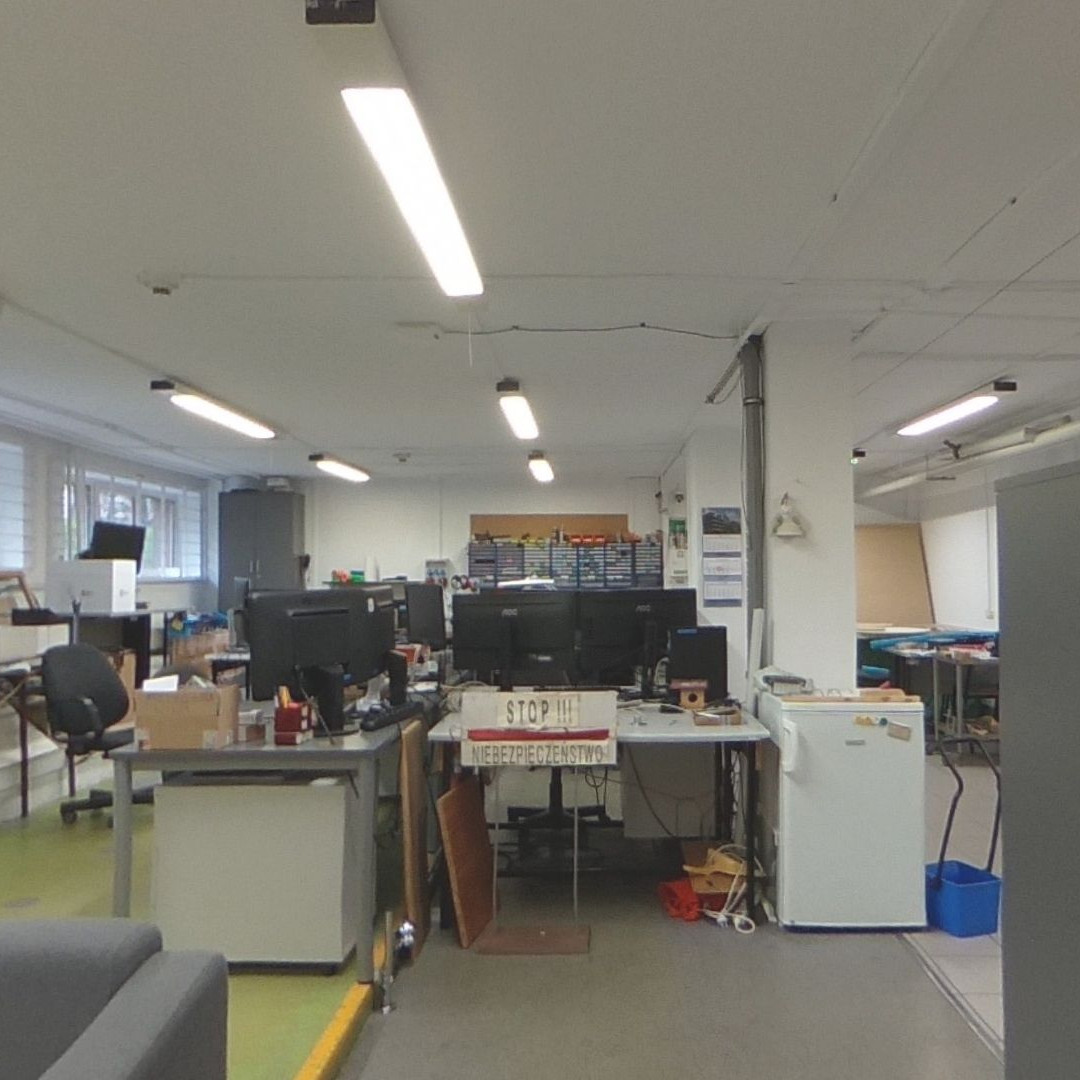
\includegraphics[width=\linewidth]{img/gazebo_vs_real/real.jpg}
        \caption{Real camera}
    \end{subfigure}\hfill%
    \begin{subfigure}{0.46\textwidth}
        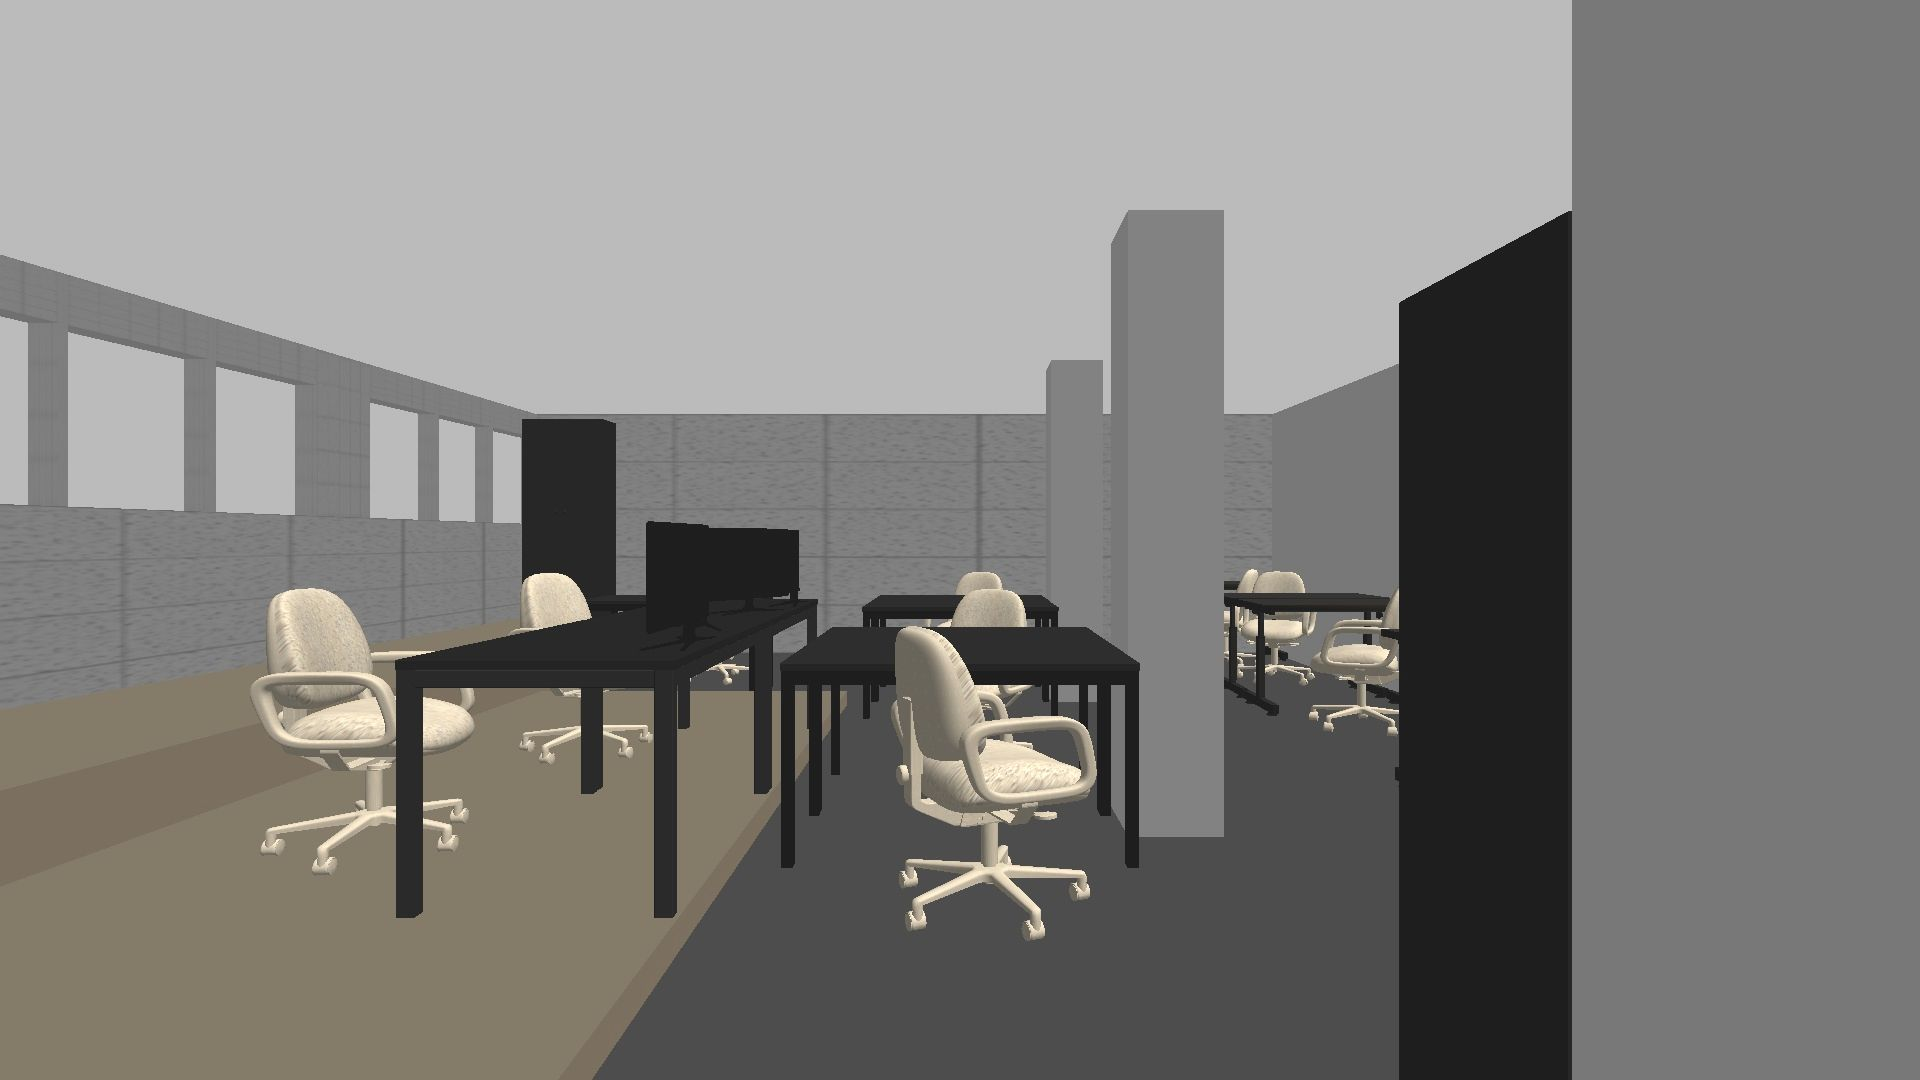
\includegraphics[width=\linewidth]{img/gazebo_vs_real/gazebo.jpg}
        \caption{Simulated camera}
    \end{subfigure}
    \caption{A comparison between a real camera and a simulated camera}
    \label{fig:gazebo_vs_real}
\end{figure}

There are some features that are desired in simulators. \cite{staranowicz2011survey}
One is the capability to quickly modify the world model used for image generation.
This allows the tester to create new test scenarios rapidly.
Another important feature is the ability to dynamically edit the robot's path.
Of course this is not possible when simulating using a prerecorded video, but should be achievable in every generic simulator as well as the capability of simulating robot's interactions with the environment such as collisions.
\begin{table}[!ht]
    \centering
    \setlength{\tabcolsep}{1em}
    \def\arraystretch{2}
    \begin{tabular}{ |c|c|c|c|c| } 
        \hline
        Feature & \textit{Gazebo} & \makecell{\textit{Pre-recorded} \\ \textit{video}} & \textit{UnrealROX} \\ 
        \hline
        \makecell{environment modification} & yes & \textbf{no} & yes \\
        \hline
        \makecell{editable robot path} & yes & \textbf{no} & yes \\
        \hline
        \makecell{interaction with \\ the environment} & yes & \textbf{no} & yes \\
        \hline
        photorealism & \textbf{no} & yes & yes \\
        \hline
        ROS integration & yes & yes & \textbf{no} \\
        \hline
    \end{tabular}
        \vspace*{1em}
        \caption{Comparison of different camera simulation methods}
        \label{tab:simulation_methods}
\end{table}

There is no method of simulating a robot's camera that has all desired features.
Specificaly, there is a need for a photorealistic simulator with ROS integration.

\subsection{Nomenclature}

A \textbf{spherical camera} is a type of camera with a field of view that covers the entire sphere and a \textbf{regular camera} is a type of camera with a field of view close to $90$ degrees.
The camera that belongs to a robot in sumulation is referred to as a \textbf{virtual camera}.
A \textbf{projection camera} is an entity that projects a 3D scene to a 2D image in computer graphics.

\section{The idea}

Images from a spherical camera can be used to photorealistically simulate an environment.
The idea is visualized on Fig. \ref{fig:flow}.

First a set of spherical images is needed.
The images are tagged with the position where each of them was taken.
The position of the virtual camera can be used to select exactly one (the closest) spherical image from the set.
A single spherical image can be transformed into a regular image using the virtual camera orientation and virtual camera parameters.
\begin{figure}[!ht]
    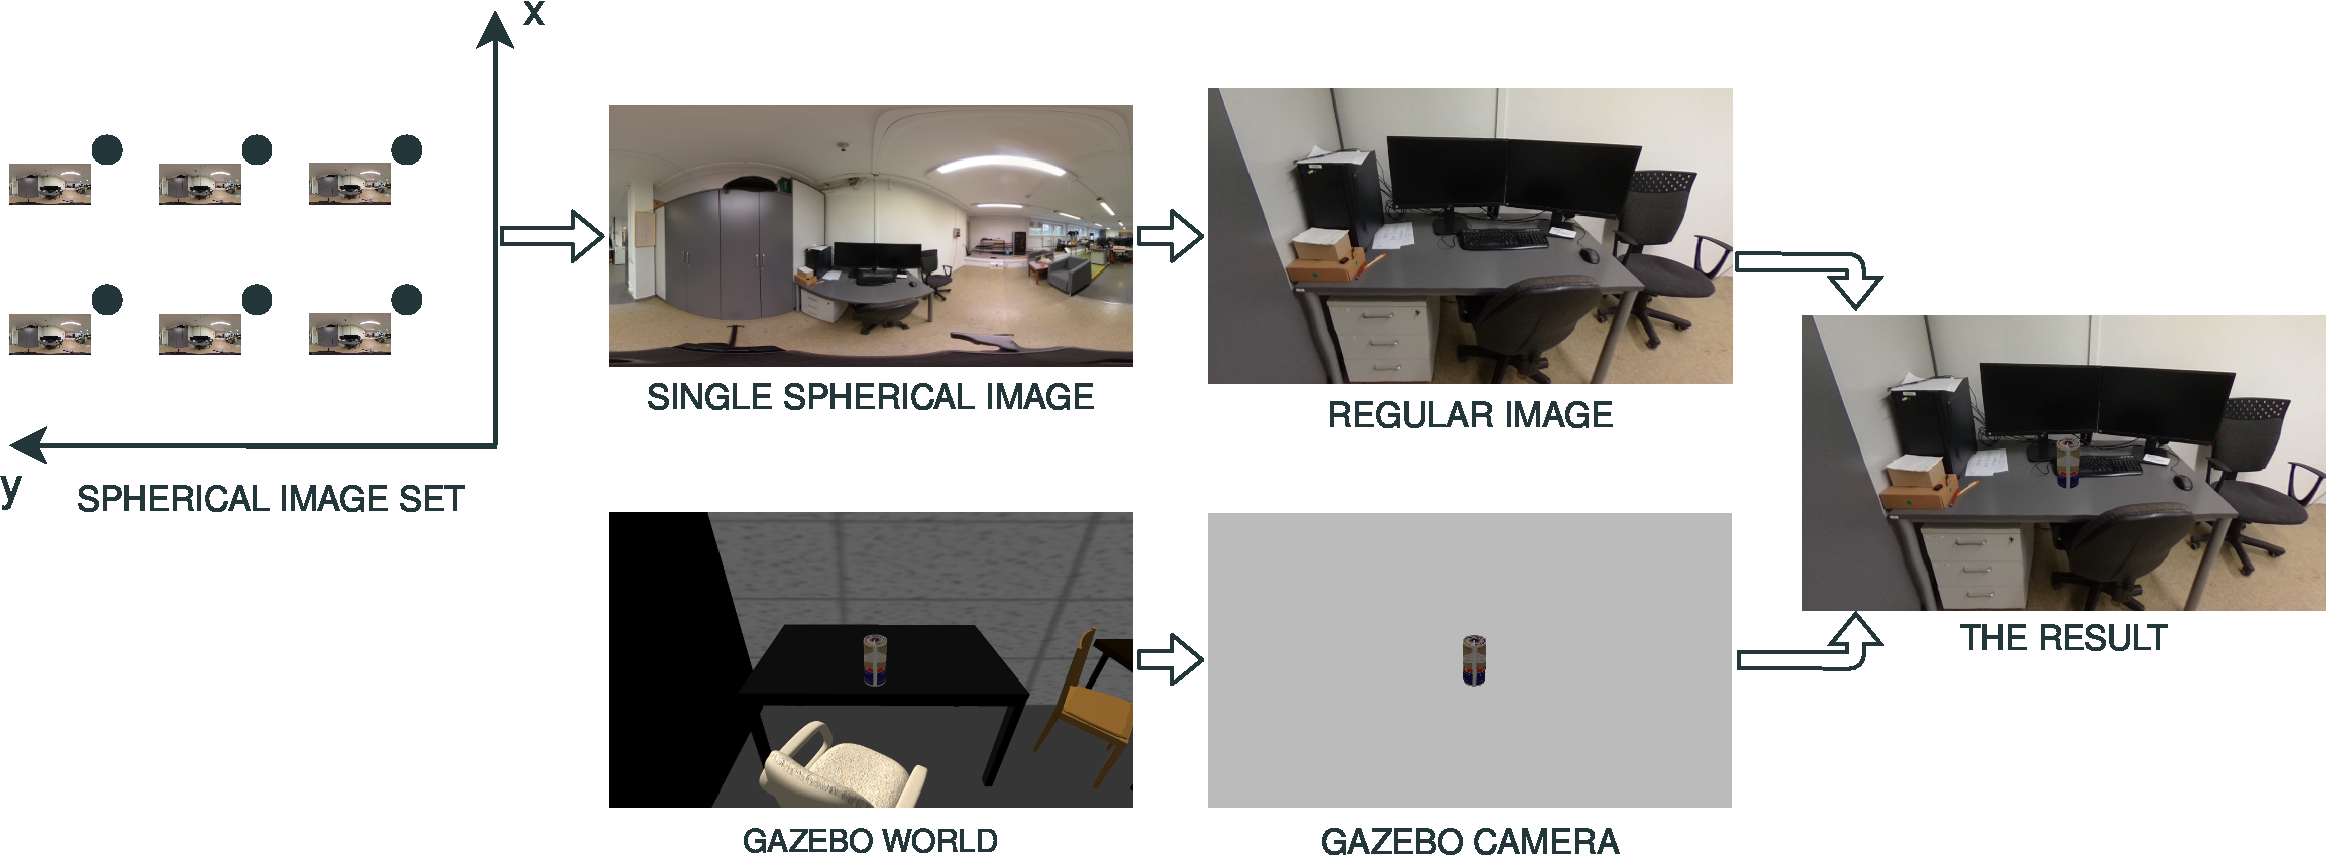
\includegraphics[width=\textwidth]{img/drawio/flow.pdf}
    \caption{The idea of the system}
    \label{fig:flow}
\end{figure}

\section{Transforming spherical images}

In order to transform a spherical image to a regular image one can utilize 3D computer graphics.
Not only is this method simple, but its implementation can utilize hardware acceleration.

A sphere is a 3D closed surface where every point on the sphere is the same distance from its origin.
The equation of a sphere with center at point $(x_0, y_0, z_0)$ and radius $R$ is as follows:
\begin{equation}
    (x - x_0)^2 + (y - y_0)^2 + (z - z_0)^2 = R^2
\end{equation}

Since only a finite number of points can be drawn, a sphere will need to be approximated by drawing a subset of its points.
Those points can be selected by creating a UV Sphere.
A UV Sphere consists of vertices that are created by performing angular steps in the spherical coordinate system.
Cartesian points are generated using these equations:
\begin{eqnarray}
    x &=& R \cdot \sin \theta \cdot \cos \varphi \\
    y &=& R \cdot \sin \theta \cdot \sin \varphi \\
    z &=& R \cdot \cos \theta
\end{eqnarray}
where $R$ is the radius of the sphere, $\theta \in [0, \pi]$ -- polar angle and $\varphi \in [0, 2\pi)$ -- azimuthal angle.

Then the sphere has to be textured with the spherical image.
Most spherical cameras create images in the form of equirectangular projections.
The process of texturing a UV sphere with an image in the form of this projection is fairly straightforward. \cite{greene1986environment} 
Every point on the sphere can be mapped to a point on the texture using the following equations:
\begin{eqnarray}
    x_t &=& R(\varphi - \varphi_0) \cos \theta_1 \\
    y_t &=& R(\theta - \theta_1)
\end{eqnarray}
where $\varphi_0$, $\theta_1$ -- center coordinates.
Those equations can be simplified by assuming $\varphi_0 = 0$ and $\theta_1 = 0$.
The sphere can also be assumed to be normalized ($R = 1$), which further simplifies the equations.
\begin{eqnarray}
    x_t &=& \varphi \\
    y_t &=& \theta
\end{eqnarray}

Having textured the sphere, now a projection camera can be placed in its center.
The image from this camera is a regular image that is the result of this transformation.

\section{Gazebo integration}

Generated images can be further processed in order to make this solution more versatile.
Namely, images from Gazebo camera can be overlaid onto those generated images in order to add objects to the simulation.
Fig. \ref{fig:join} depicts an example of such process.
This provides additional simulation features mentioned in the introduction.
It enables the tester to modify the testing environment and provides the means of interaction of the simulated robot with the environment by the means of the Gazebo simulator.
\begin{figure}[!ht]
    \centering
    \begin{subfigure}{.46\textwidth}
        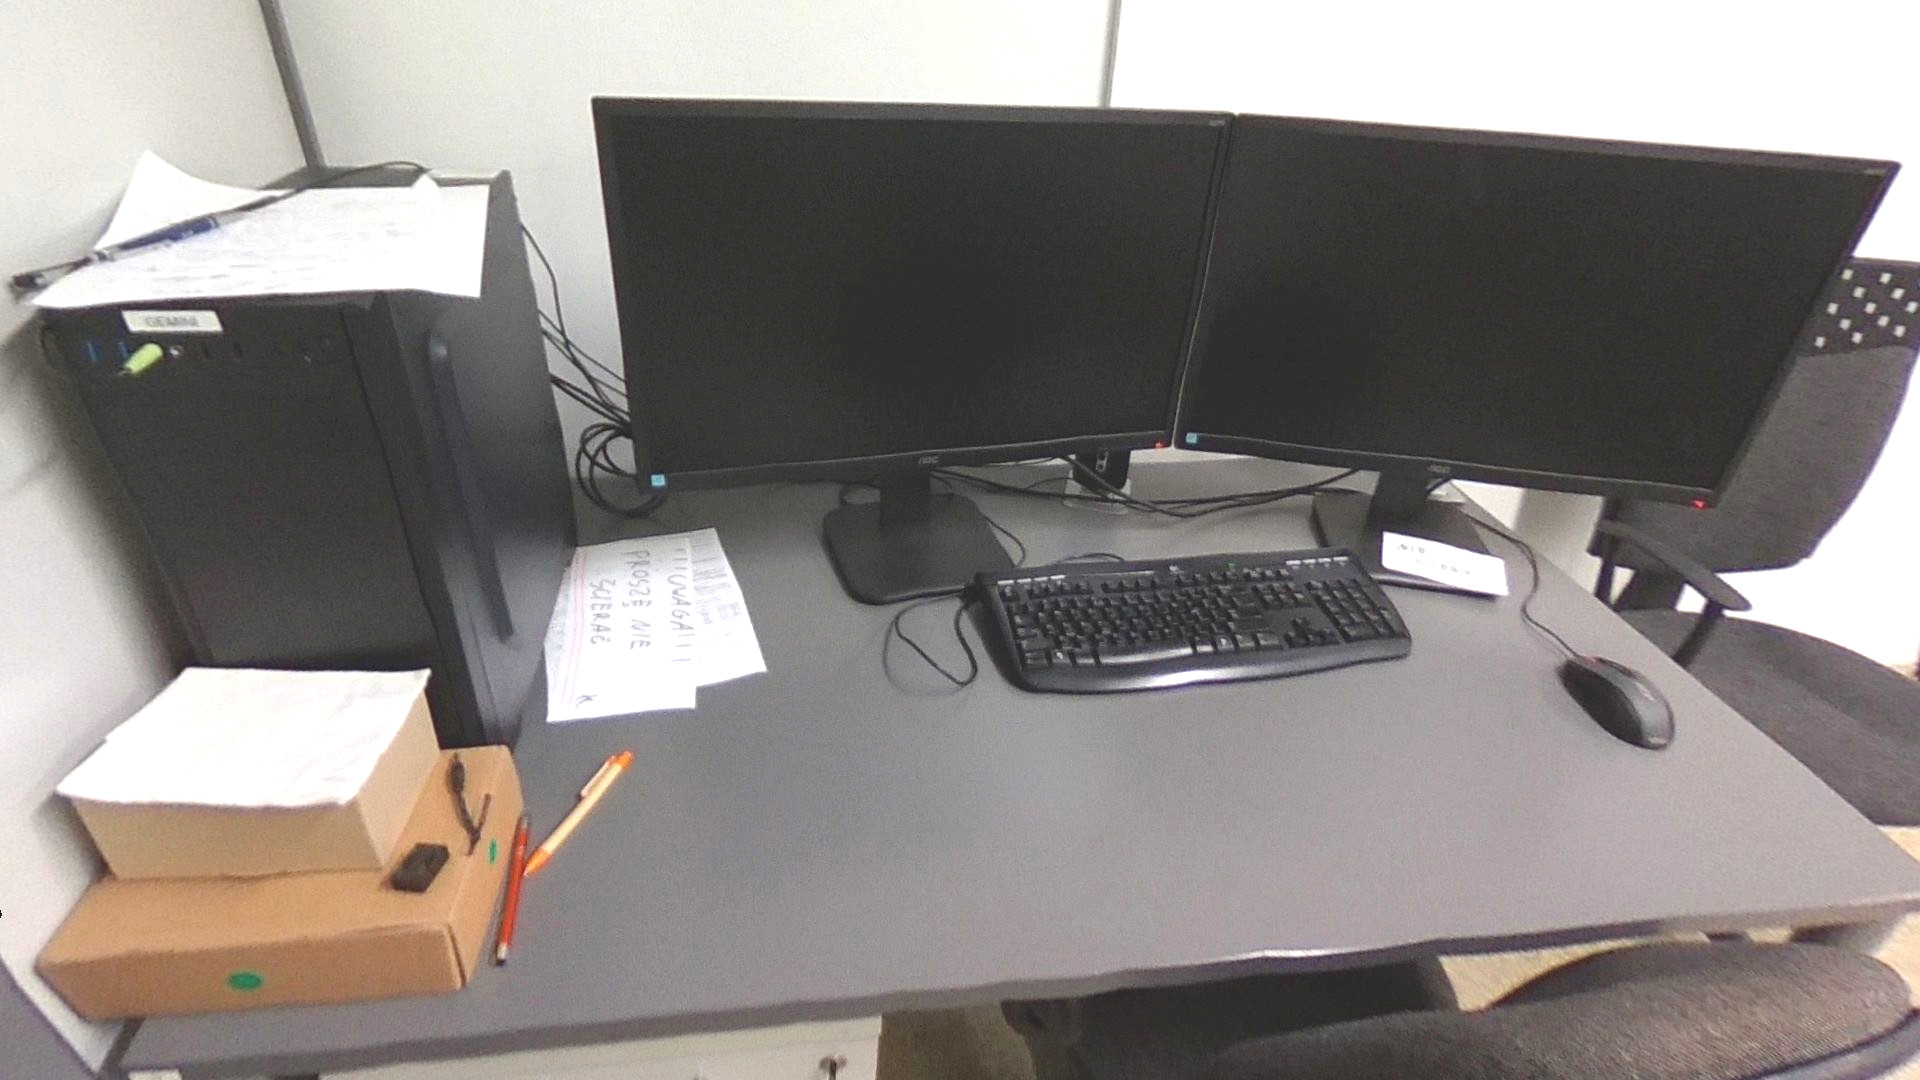
\includegraphics[width=\linewidth]{img/gazebo_integration/sim.jpg}
        \caption{Image generated from a spherical image}
        \vspace*{1em}
    \end{subfigure}\hfill%
    \begin{subfigure}{.46\textwidth}
        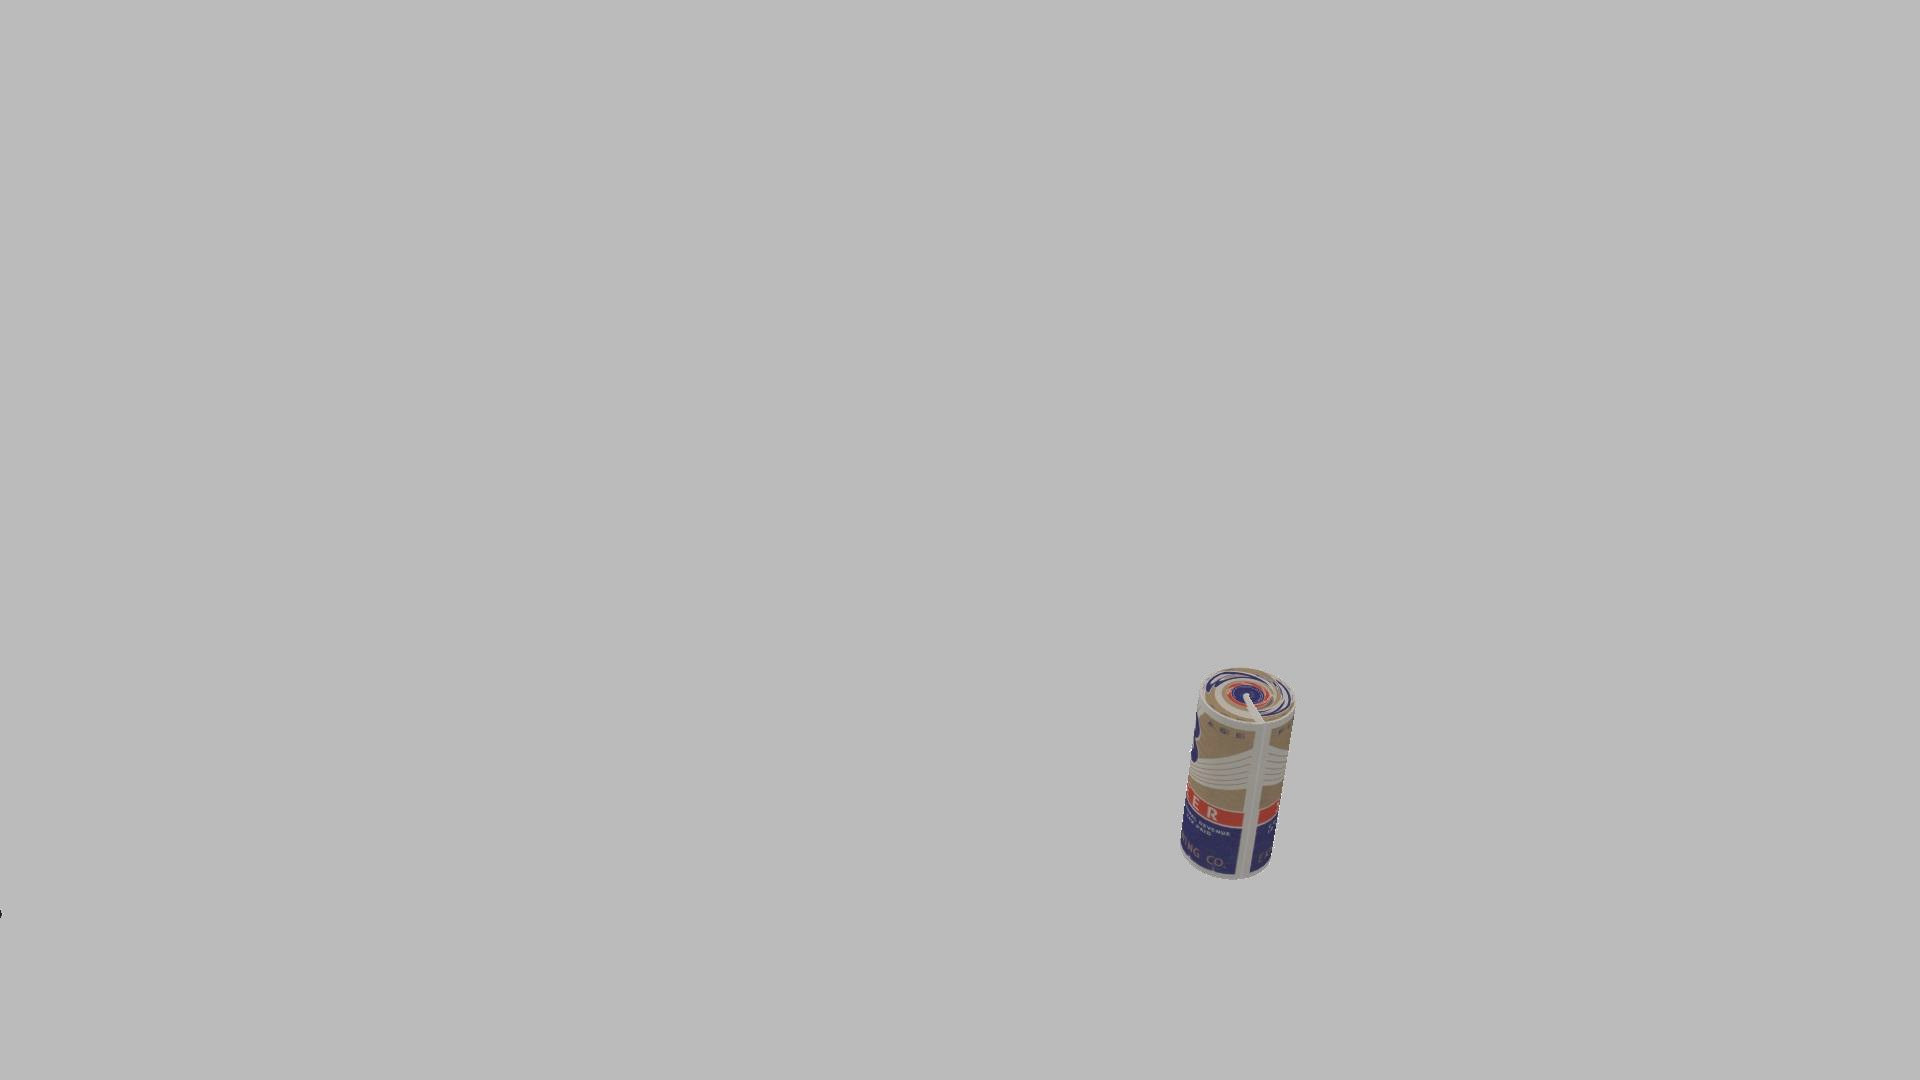
\includegraphics[width=\linewidth]{img/gazebo_integration/gazebo.jpg}
        \caption{Image from Gazebo camera}
        \vspace*{1em}
    \end{subfigure}
    \begin{subfigure}{\textwidth}
        \centering
        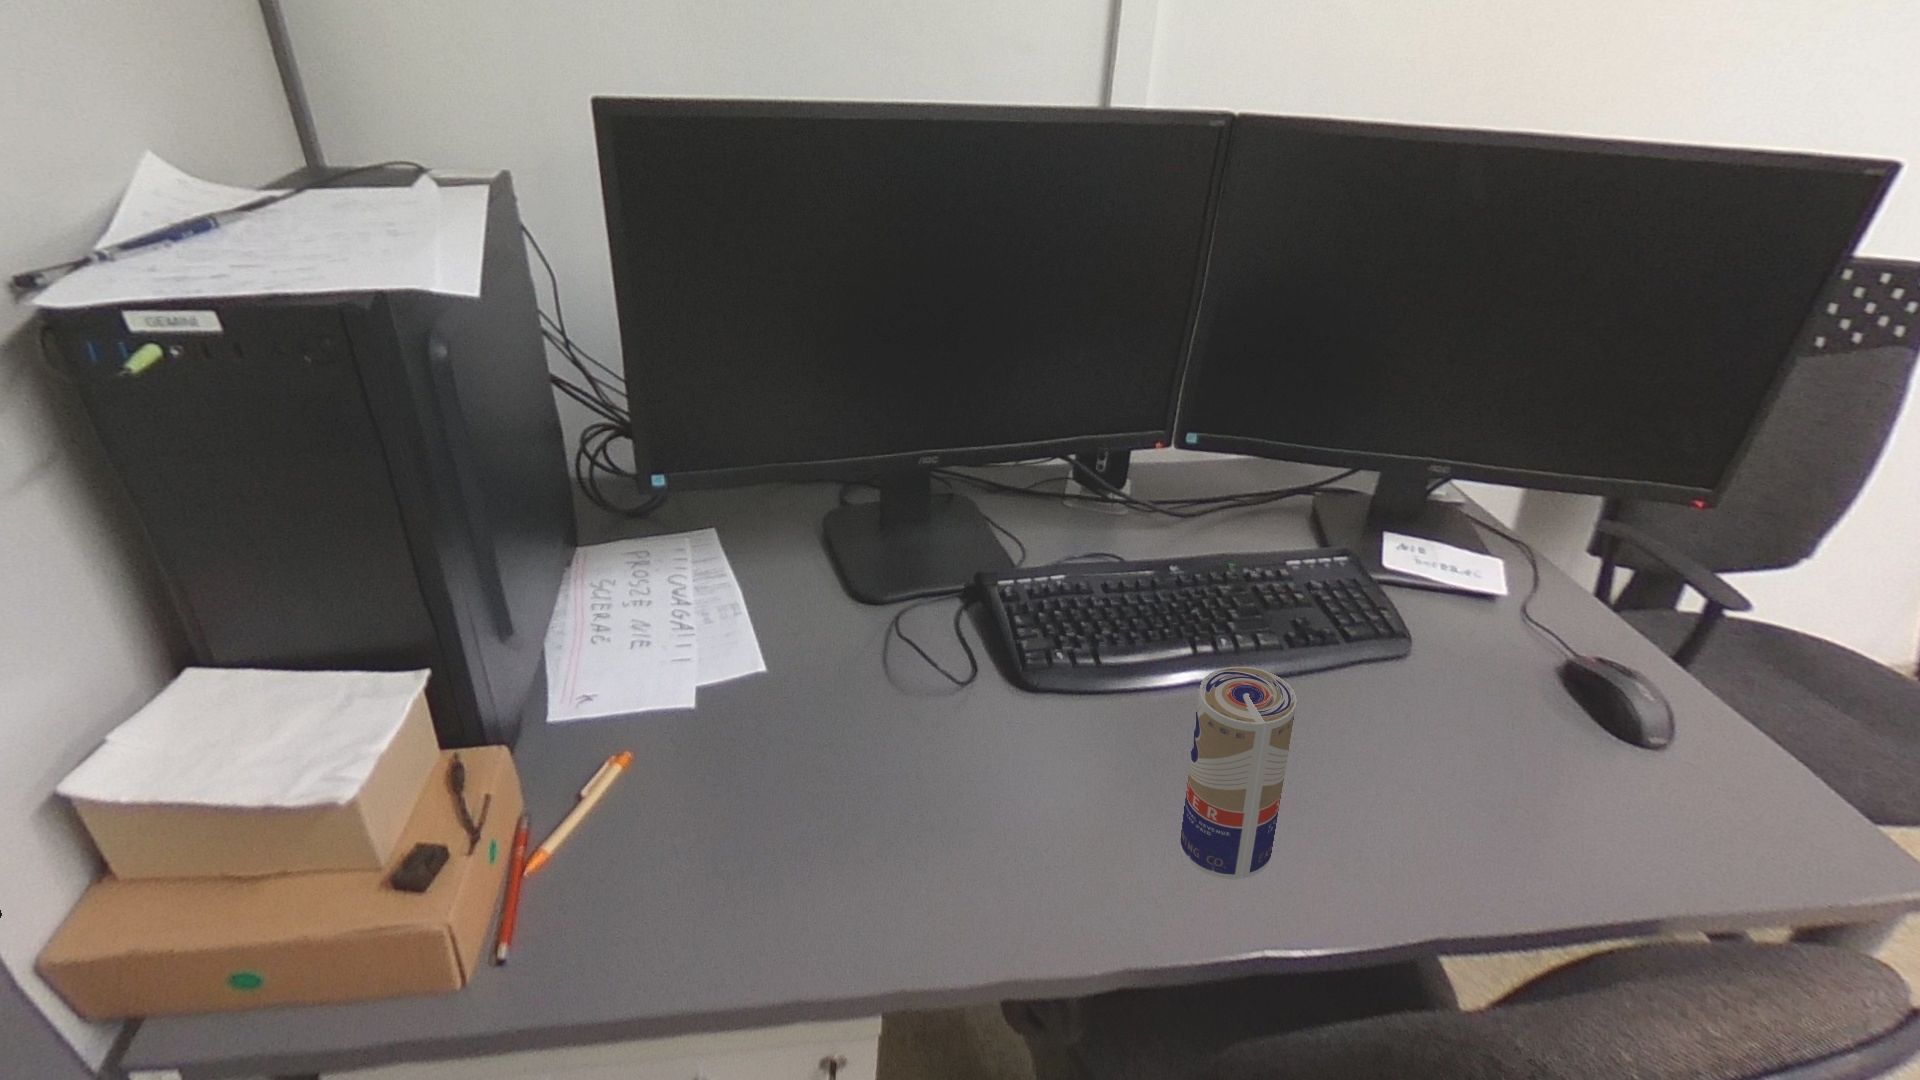
\includegraphics[width=0.5\linewidth]{img/gazebo_integration/sum.jpg}
        \caption{The result}
    \end{subfigure}
    \caption{Adding virtual objects to generated images}
    \label{fig:join}
\end{figure}

\section{Interpolation}

The fact that always the nearest spherical image is used for rendering poses a significant issue.
This problem is visualized on Fig. \ref{fig:interpolation_problem}.
\begin{figure}[!ht]
    \centering
    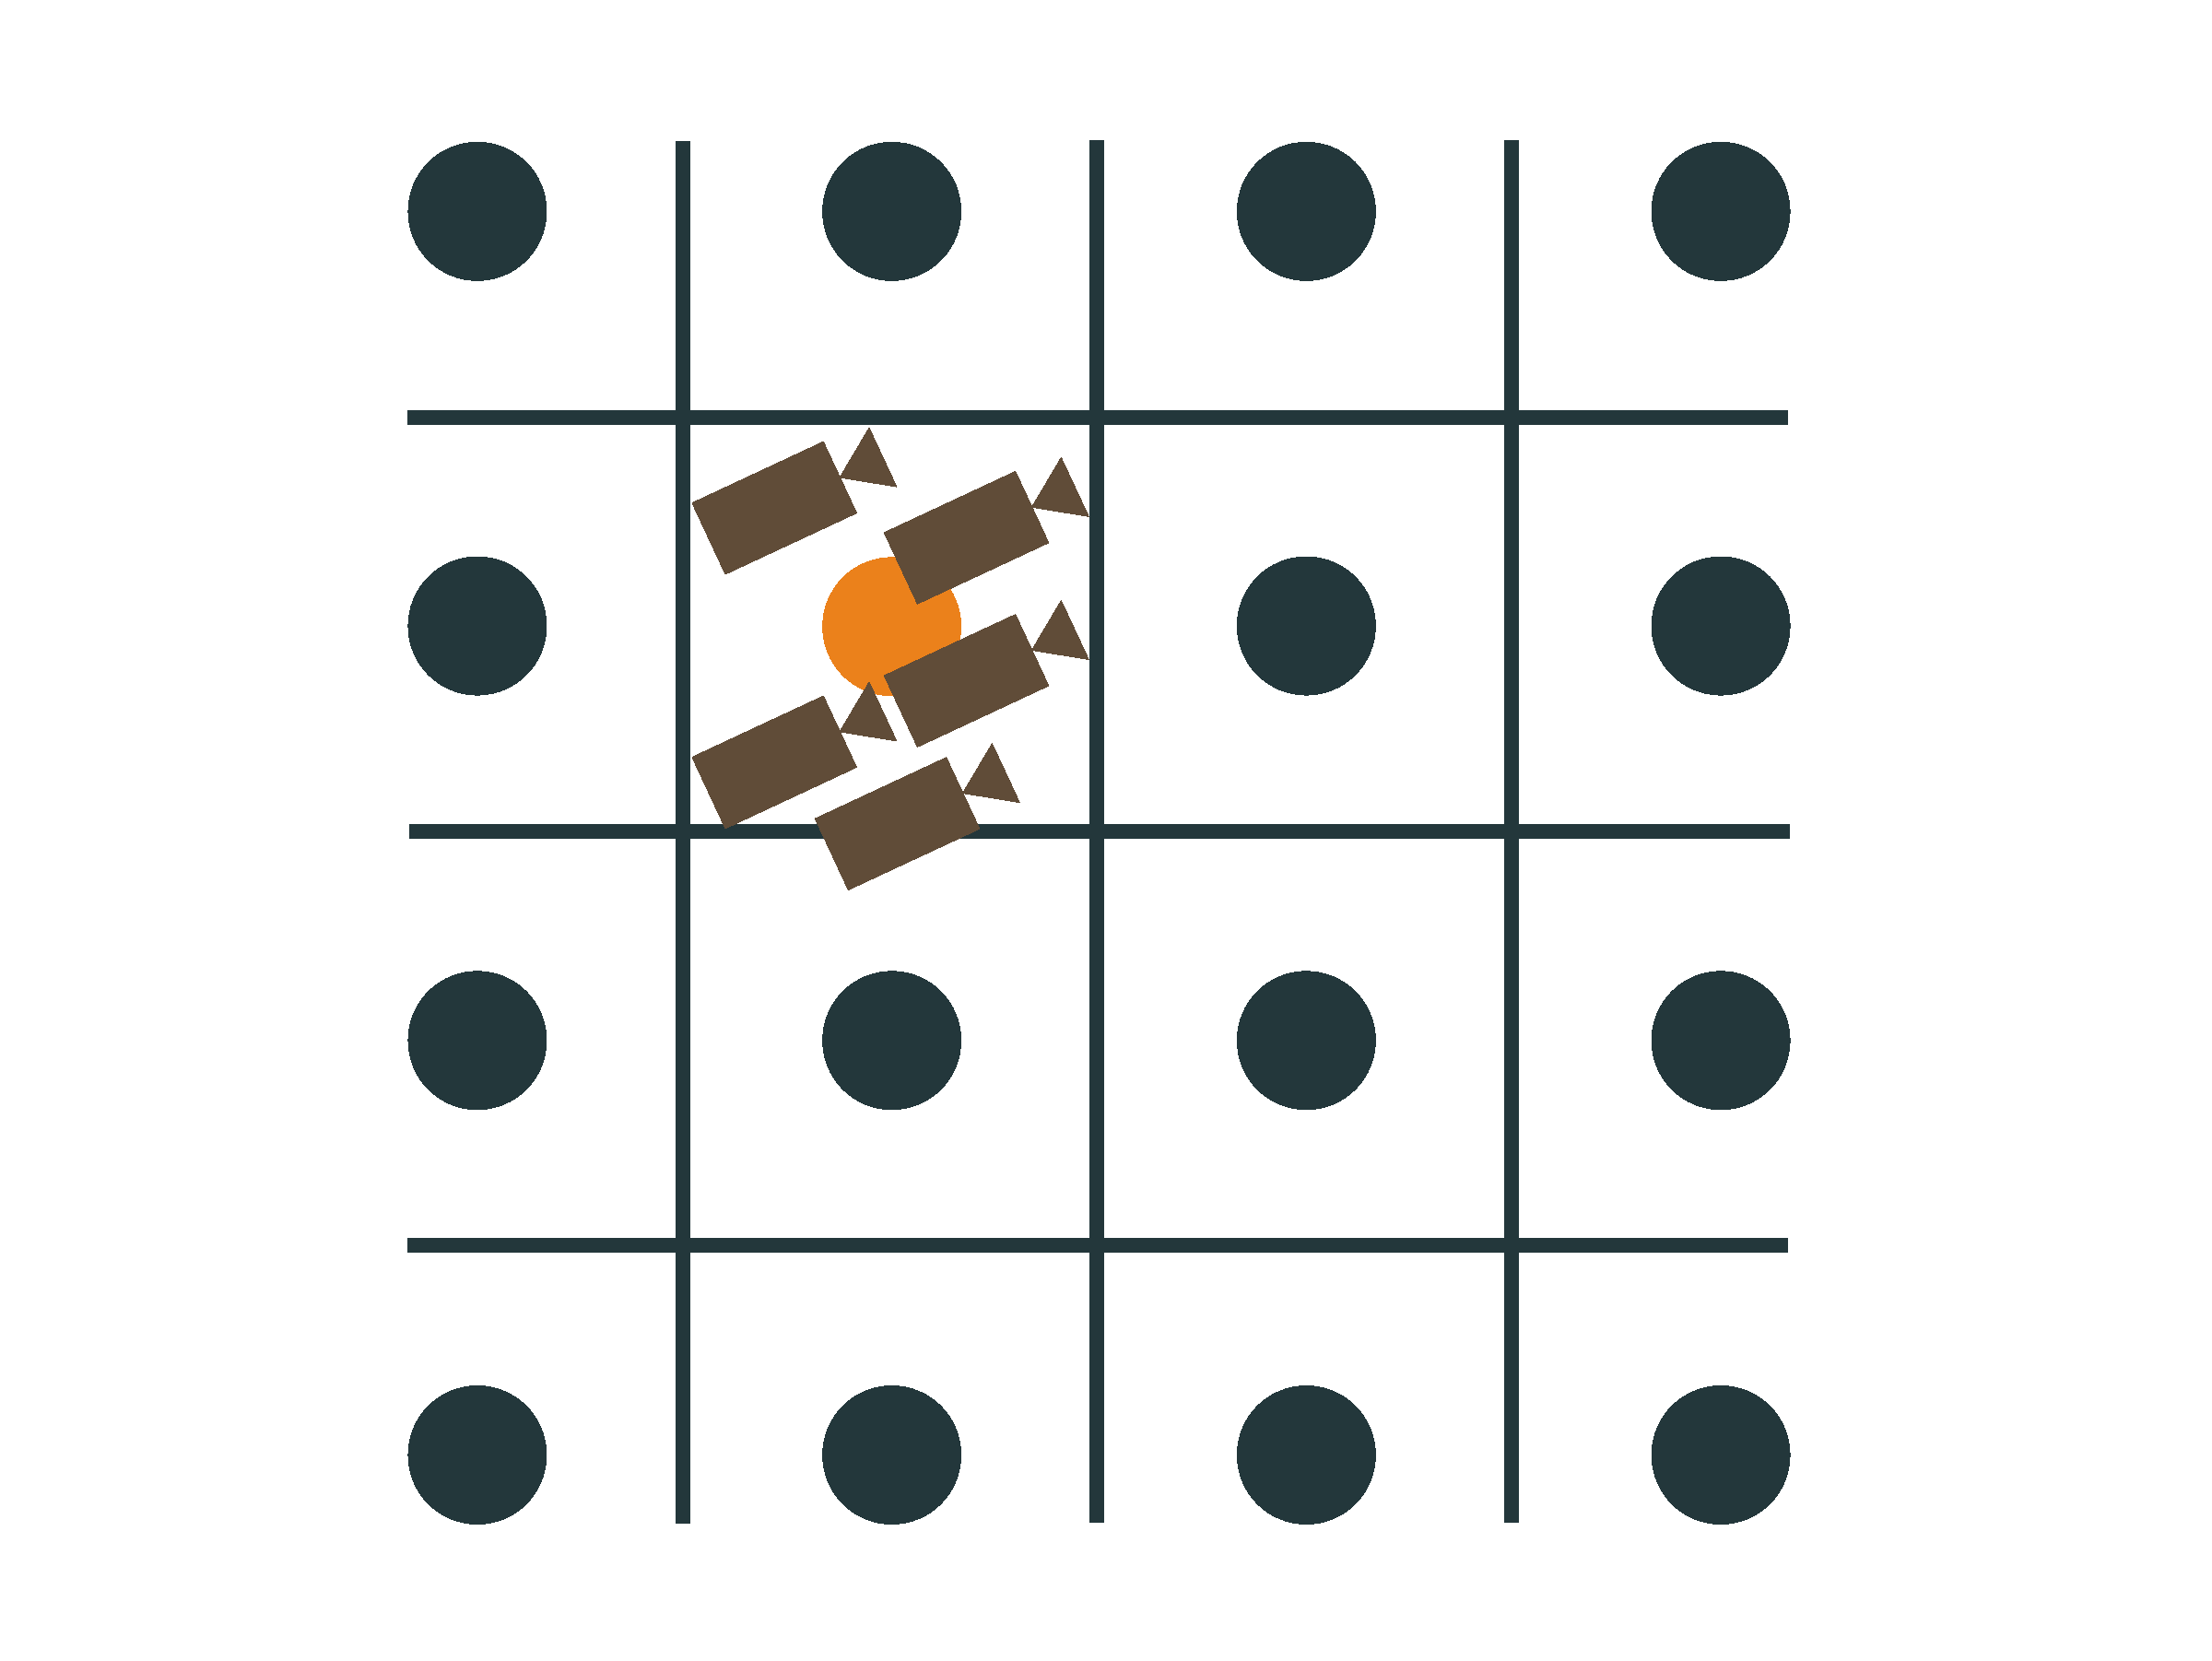
\includegraphics[width=0.75\textwidth]{img/drawio/interpolation-1.pdf}
    \caption{Problematic arrangement resulting in identical generated images}
    \label{fig:interpolation_problem}
\end{figure}

The dots represent the set of spherical images (top-down view) and the grid divides the surface into regions tied to a spherical image at its center.
Camera icons symbolize exemplary positions and orientations of virtual cameras with equal parameters.
All cameras use the same spherical image for simulation (the closest image is marked orange).
Moreover, all cameras have the same orientation relative to the global reference frame.
This means that the same regular image would be produced for all the cameras.

A simple solution to this problem would be to mimic the position of the virtual camera relative to a region with the position of the projection camera thus creating the ilusion of moving closer to certain objects as visualized in Fig. \ref{fig:interpolation}.
\begin{figure}[!ht]
    \begin{subfigure}{\textwidth}
        \centering
        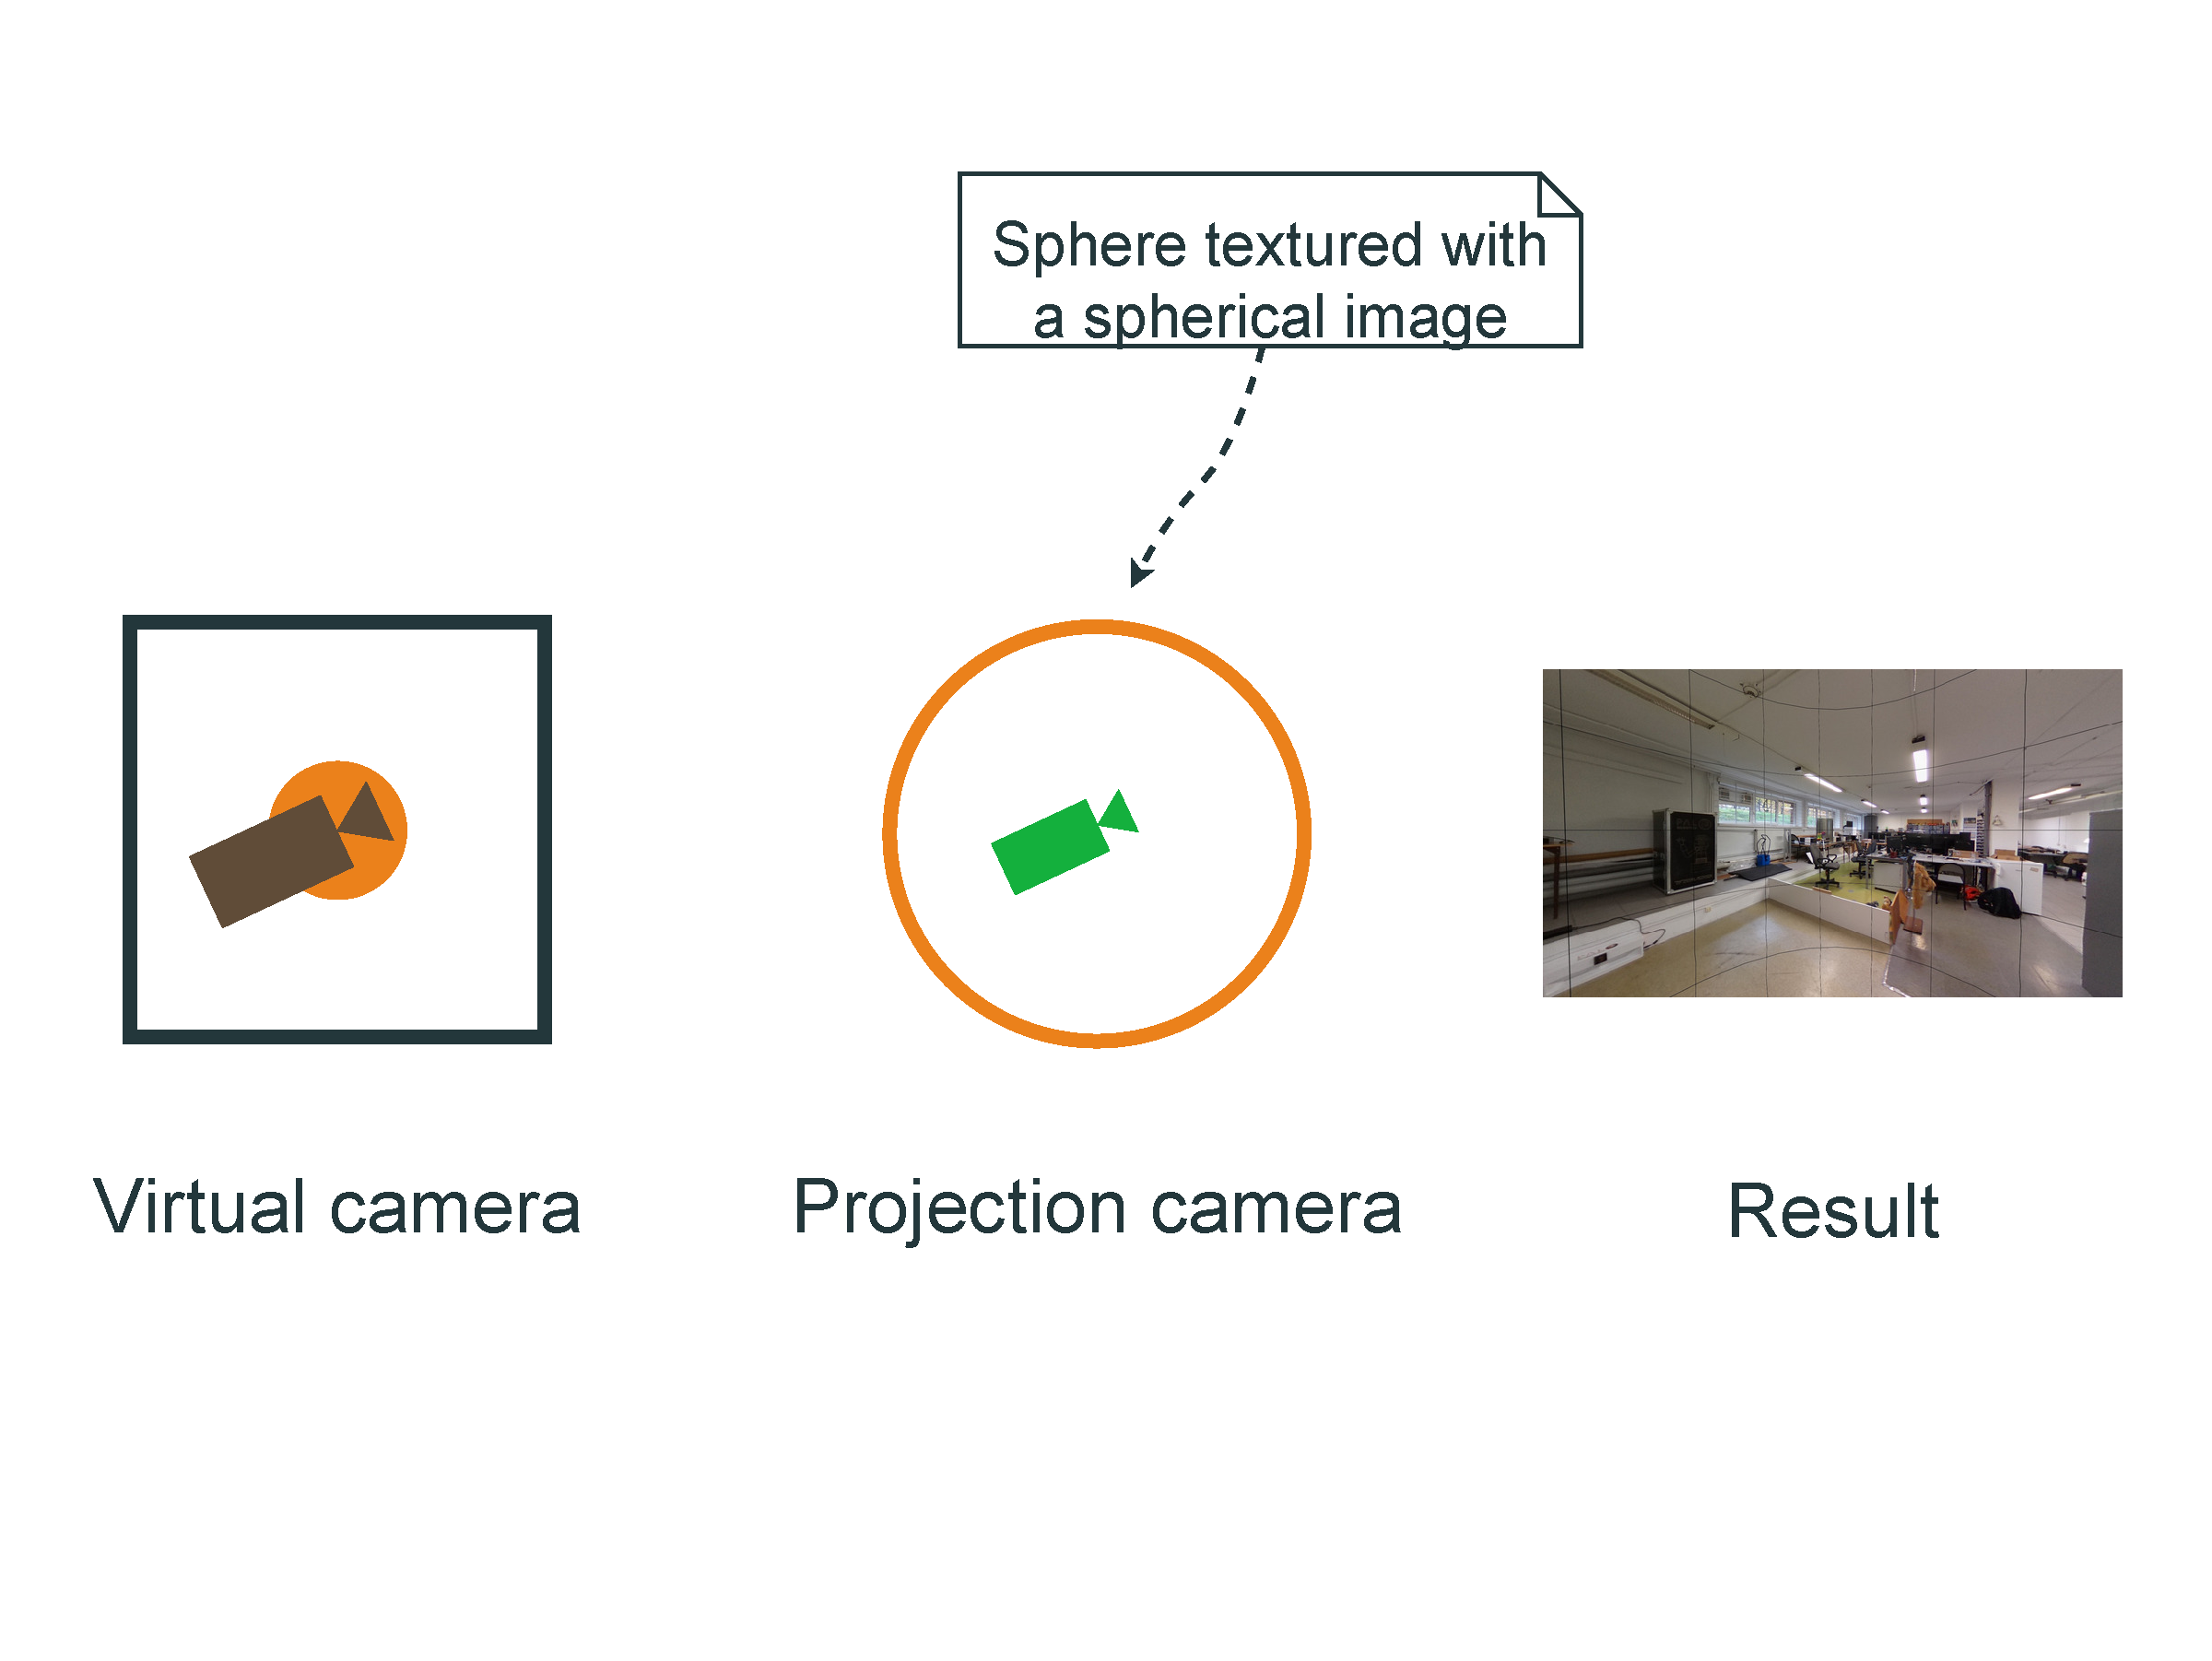
\includegraphics[width=0.9\linewidth]{img/drawio/interpolation-2.pdf}
        \caption{}
        \label{fig:interpolation1}
    \end{subfigure}
    \begin{subfigure}{\textwidth}
        \centering
        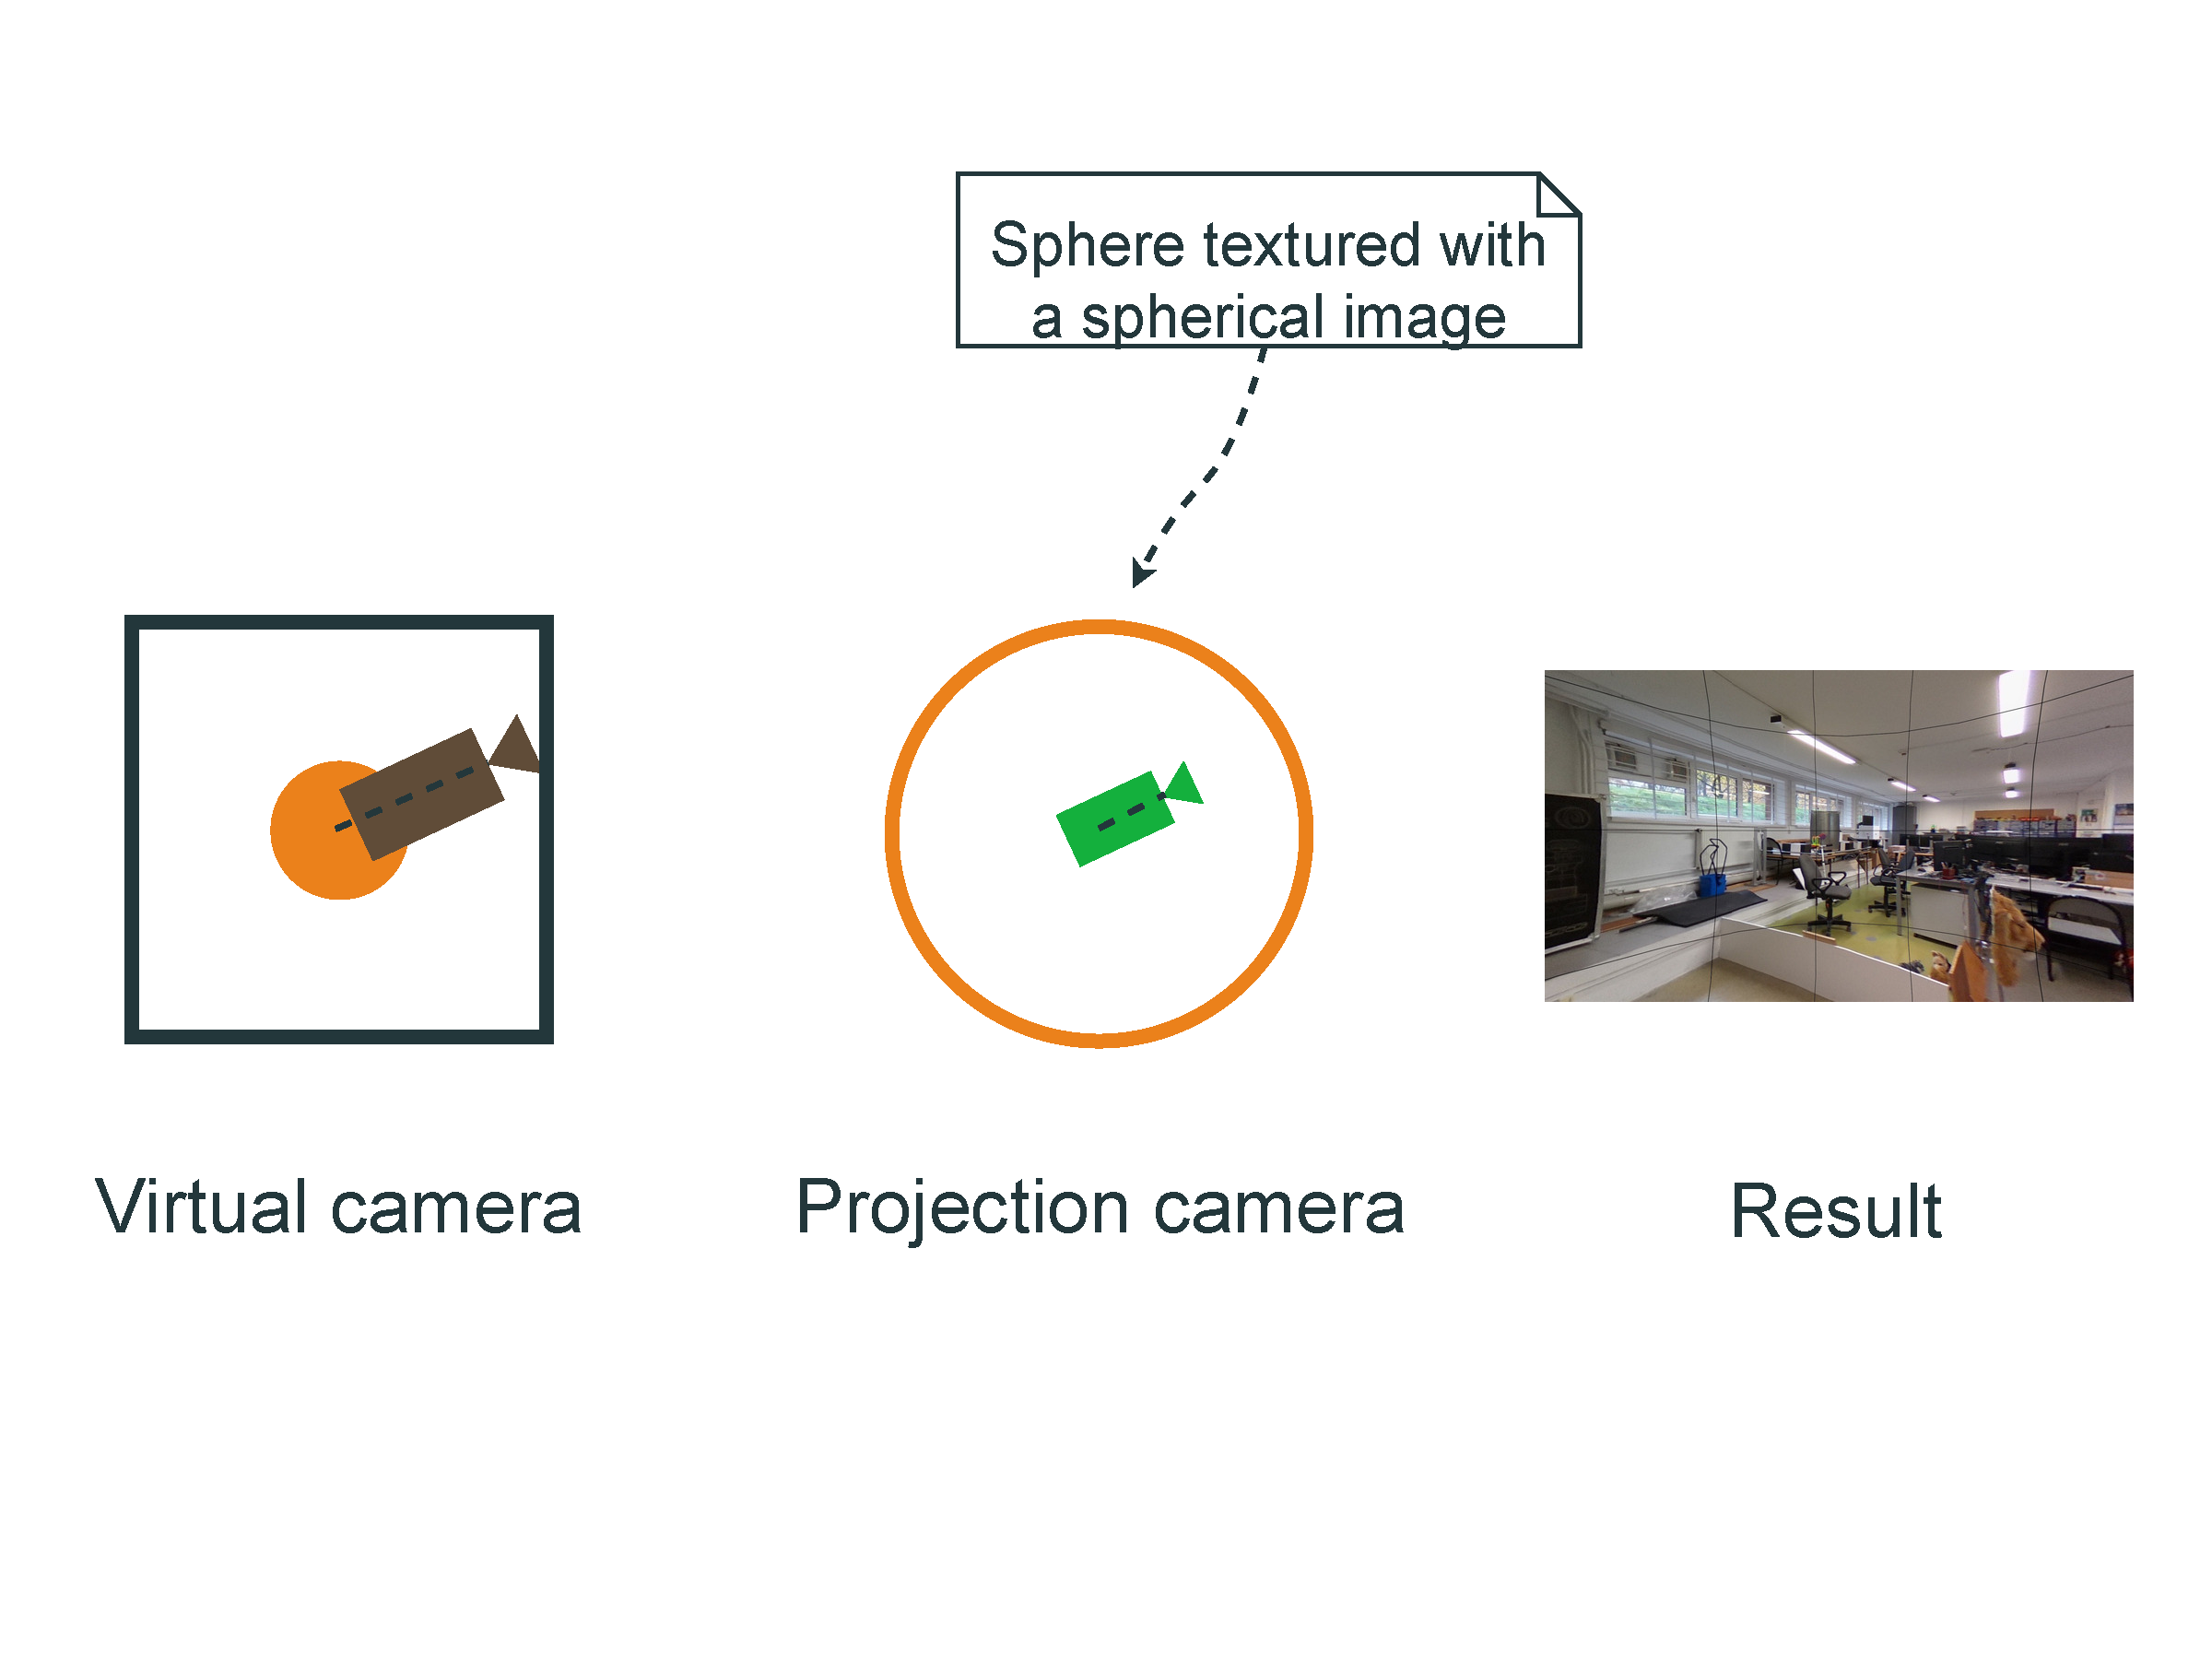
\includegraphics[width=0.9\linewidth]{img/drawio/interpolation-3.pdf}
        \caption{}
        \label{fig:interpolation2}
    \end{subfigure}
    \caption{The method of interpolating camera views}
    \label{fig:interpolation}
\end{figure}

\section{A set of spherical images}

A set of spherical images can be created using hardware like shown on Fig. \ref{fig:rig}.
It consists of a rail and a cart to which a monopod has been fixed.
At the other end of the monopod there is a mounting system for the camera.
A graduation was applied to the rail in order to allow precise positioning of the cart.
In order to guide the rail, a graduation was also applied to the floor.
\begin{figure}[!ht]
    \centering
    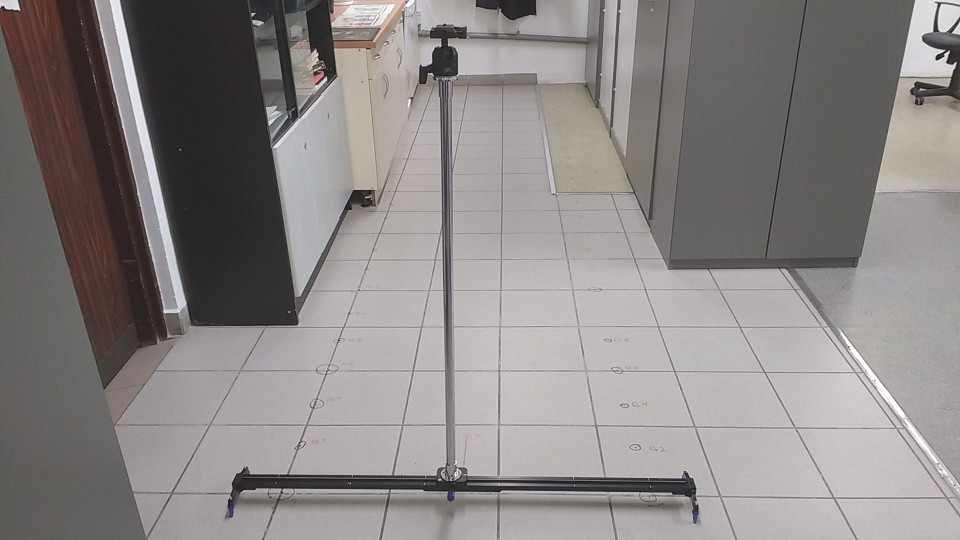
\includegraphics[width=0.75\textwidth]{img/rig/calosc.jpg}
    \caption{Hardware used for the creation of the image set}
    \label{fig:rig}
\end{figure}
In the chosen room 404 pictures were taken in $20 cm$ intervals.
The whole process lasted 2 hours 17 minutes and 20 seconds, which yields approximately 20 seconds for one picture or 3 pictures a minute.

In the process of taking pictures, to simplify keeping track of the areas already covered with spherical images, an application was created (Fig. \ref{fig:app}).
The application allows selecting points and making requests of taking pictures to the camera.
It also automatically tags images with the correct position.
\begin{figure}[!ht]
    \centering
    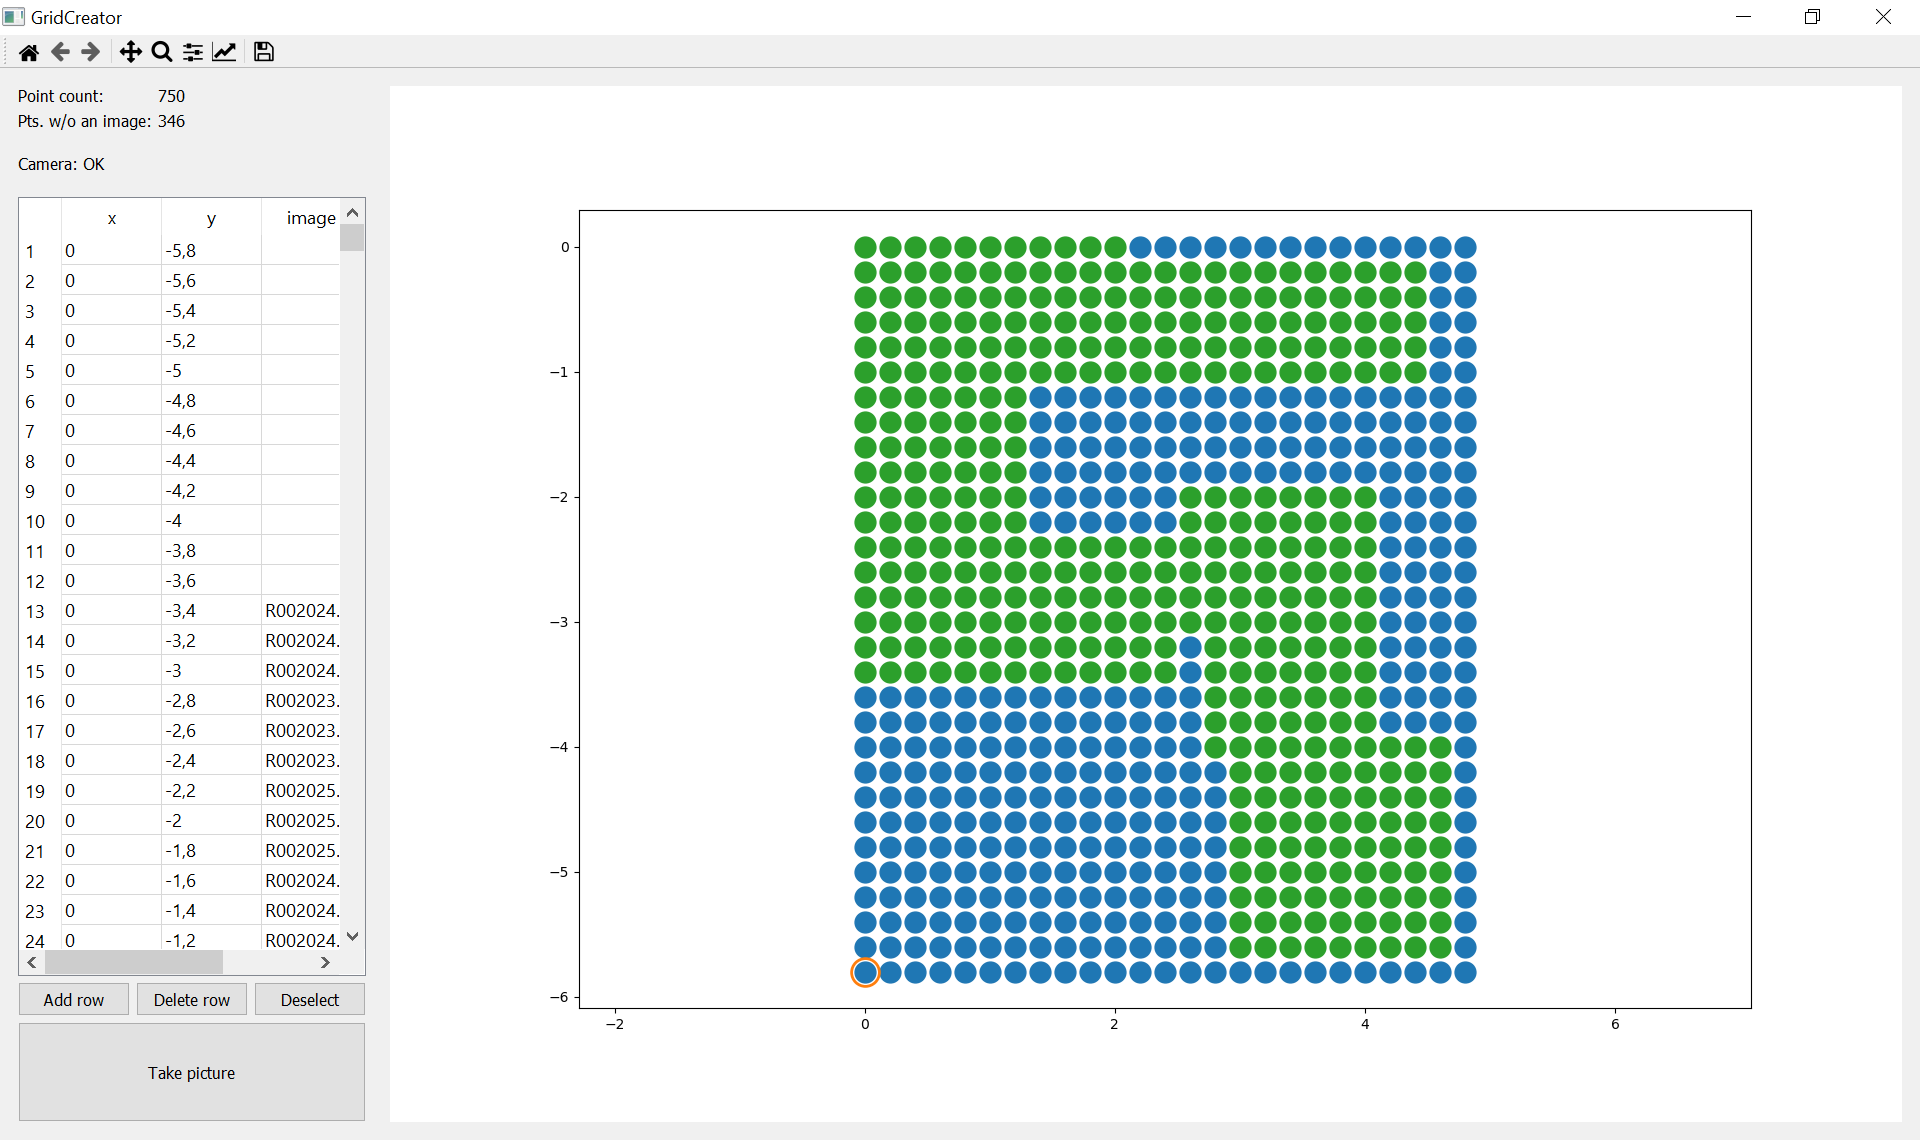
\includegraphics[width=0.75\textwidth]{img/creator.png}
    \caption{Application created to aid in image set creation}
    \label{fig:app}
\end{figure}

\section{Evaluation}

The whole solution was evaluated by comparing generated images with images from a real robot.
For this purpose the TIAGo robot was used.
It was booted up and manually controlled in order to take pictures.
Then the proposed solution was used to generate images corresponding to pictures taken by TIAGo.
Finally, images from both sources were compared as seen on Fig. \ref{fig:sim_vs_tiago}.

\begin{figure}[!ht]
    \centering
    \begin{subfigure}{0.46\textwidth}
        \centering
        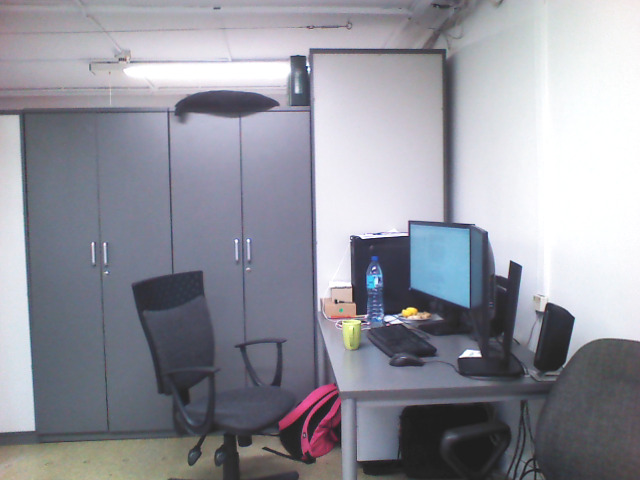
\includegraphics[width=\linewidth]{img/sim_vs_tiago/tia_biurko.jpg}
        \caption{}
        \vspace*{1em}
    \end{subfigure}\hfill%
    \begin{subfigure}{0.46\textwidth}
        \centering
        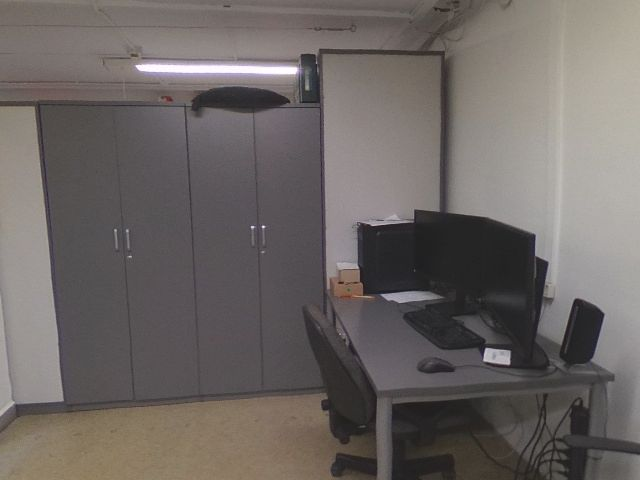
\includegraphics[width=\linewidth]{img/sim_vs_tiago/sim_biurko.jpg}
        \caption{}
        \vspace*{1em}
    \end{subfigure}
    \begin{subfigure}{0.46\textwidth}
        \centering
        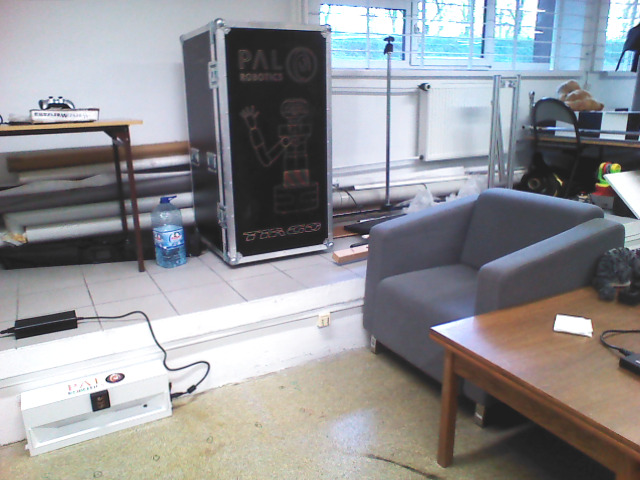
\includegraphics[width=\linewidth]{img/sim_vs_tiago/tia_fotel.jpg}
        \caption{}
        \vspace*{1em}
    \end{subfigure}\hfill%
    \begin{subfigure}{0.46\textwidth}
        \centering
        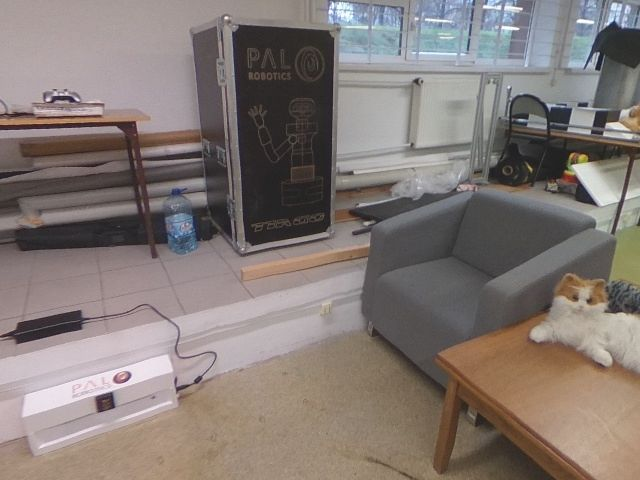
\includegraphics[width=\linewidth]{img/sim_vs_tiago/sim_fotel.jpg}
        \caption{}
        \vspace*{1em}
    \end{subfigure}
    \begin{subfigure}{0.46\textwidth}
        \centering
        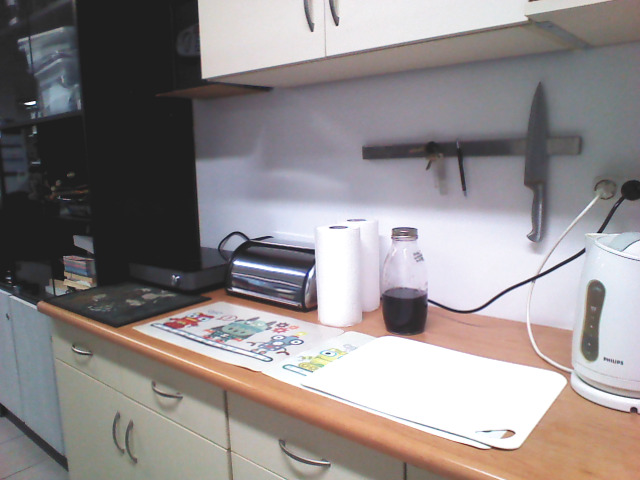
\includegraphics[width=\linewidth]{img/sim_vs_tiago/tia_kuchnia_blat.jpg}
        \caption{}
        \vspace*{1em}
    \end{subfigure}\hfill%
    \begin{subfigure}{0.46\textwidth}
        \centering
        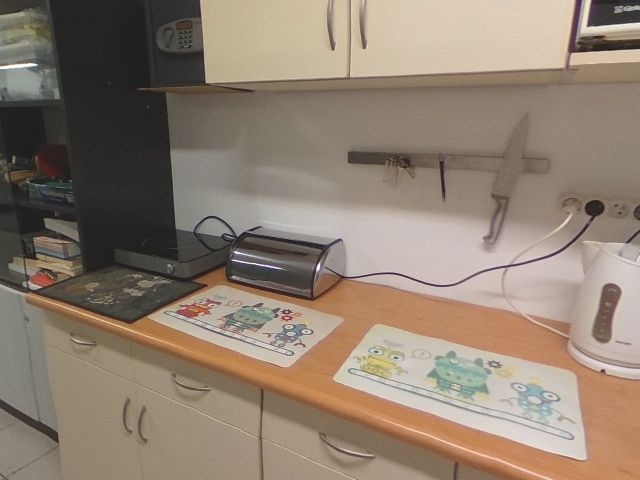
\includegraphics[width=\linewidth]{img/sim_vs_tiago/sim_kuchnia_blat.jpg}
        \caption{}
        \vspace*{1em}
    \end{subfigure}
    \caption{Images taken by TIAGo (left) and images from a virtual camera (right)}
    \label{fig:sim_vs_tiago}
\end{figure}

The images differ mainly in color appearance and are otherwise nearly identical.
The mentioned color issue can be resolved by the means of color correction.
Those results prove that using the proposed solution a set of spherical images can be used to replace a real robot in software testing.

\clearpage

\nocite{*}
\bibliographystyle{unsrt}
\bibliography{bibliography}

\end{document}
